\documentclass[PST,authoryear,toc]{lsstdoc}
% lsstdoc documentation: https://lsst-texmf.lsst.io/lsstdoc.html
\input{meta}
\usepackage{placeins}

% Package imports go here.

% Local commands go here.

%If you want glossaries
%\input{aglossary.tex}
%\makeglossaries
\newcommand{\rband}{\ensuremath{r}-band}

\newcommand{\cm}{\ensuremath{C_m}}
\newcommand{\mf}{\ensuremath{m_5}}
\newcommand{\fsig}{\ensuremath{5\sigma}}
\newcommand{\texp}{\ensuremath{t_{\rm{vis}}}}
\newcommand{\baseline}{\texttt{baseline\_v2.0}}
\newcommand{\fwhme}{\ensuremath{{\rm FWHM}_\mathrm{Eff}}}

%\newcommand{\SRD}{\href{https://docushare.lsst.org/docushare/dsweb/Get/LPM-17}{\textcolor[HTML]{1155CC}{SRD}}}

\setlength\parindent{10pt}

\renewcommand{\arraystretch}{1.3}



\title{Updated estimates of the Rubin system throughput and expected LSST image depth}


% Optional subtitle
% \setDocSubtitle{A subtitle}

\input{authors}
\date{February 2022}

\setDocRef{PSTN-054}
\setDocUpstreamLocation{\url{https://github.com/lsst-pst/pstn-054}}

\date{\vcsDate}

% Optional: name of the document's curator
% \setDocCurator{The Curator of this Document}

\setDocAbstract{%
This document presents updated estimates, as of May 2022, of the Rubin system throughput and compares them to throughput requirements from the LSST Science Requirements Document. In addition, it uses these estimates to forecast LSST’s median single-visit and
co-added image depths for the current (OpSim v2.0) baseline LSST cadence simulation:
(23.8, 24.5, 24.0, 23.4, 22.7, 22.0) and (25.6, 26.9, 26.9, 26.4, 25.6, 24.8) in
$ugrizy$, respectively.
In addition, it uses these estimates to
forecast LSST’s median single-visit and co-added image depths for the current baseline LSST cadence simulation. Estimated system performance relies on actual measurements of the performance of various system
hardware components, and on simulations where measurements are still unavailable. The updated performance estimates meet all the relevant requirements from the LSST Science Requirements Document.
As our knowledge of the as-buit system continues to improve, updates to these estimates will continue to be provided.
}

% Change history defined here.
% Order: oldest first.
% Fields: VERSION, DATE, DESCRIPTION, OWNER NAME.
% See LPM-51 for version number policy.
\setDocChangeRecord{%
  \addtohist{1}{YYYY-MM-DD}{Unreleased.}{federica bianco (she/her/hers)}
}


\begin{document}

% Create the title page.
\maketitle
% Frequently for a technote we do not want a title page  uncomment this to remove the title page and changelog.
% use \mkshorttitle to remove the extra pages

% ADD CONTENT HERE

\section{Introduction}

The LSST System Science Requirements Document (\citeds{LPM-17}, hereafter SRD) lists the science-driven requirements for the data products to be delivered by LSST.
Engineering requirements for each technical subsystem of the Rubin Observatory have been derived from this document.

The required overall system throughput is specified by requirements listed in the SRD Tables 5 and 6 (also reported in Table 1 of \citet{2019ApJ...873..111I}).
Those requirements primarily constrain the effective primary mirror diameter and overall (hardware $+$ atmosphere)
system throughput ({\it e.g.}, mirror surface reflectivity, sensor quantum efficiency). For ease of interpretation,
Tables 5 and 6 express these requirements in terms of limiting image depth, \mf\ (defined as a magnitude at which
a photometric signal-to-noise ratio SNR=5 is attained), corresponding to {\bf fiducial} observing parameters. These fiducial parameters
include exposure time per visit (2$\times$15 sec), delivered $r$-band seeing (0.7 arcsec), boresight airmass ($X=1$) and $r$-band sky brightness (14.5 mJy arcsec$^{-2}$, equivalent to
21 AB mag arcsec$^{-2}$).

While these fiducial values were chosen to approximately correspond to realistic observing conditions, the \mf\ values listed in Tables 5 and 6 should {\bf not} be interpreted as expected LSST single-visit depths (for example,
the telescope cannot even point towards the zenith such that $X>1$ for all observations, and the fiducial sky brightness is approximately equivalent to
astronomical {\it dark} sky brightness). In \autoref{sec:SRD} we derive the relevant quantities related to the SRD requirements with updated system and hardware component information. To predict the single-visit depth distribution and co-added image depth,
cadence simulations that account for the variation of anticipated observing conditions are needed. These simulations are discussed
in \autoref{sec:cadence}. Finally, we discuss potential venues for optimization of the hardware elements and survey and the impact they would have on image depth in \autoref{sec:optimize}.

\section{Comparison of current throughput estimates with the SRD requirements \label{sec:SRD}}

Given the measured or assumed performance of various system hardware components (including transmissivity and reflectivity
for optical components, quantum efficiency for sensors, instrumental noise) and the fiducial observing
parameters listed in the previous section, the corresponding limiting image depth is computed using a procedure
described in
\citeds{LSE-40}
and version-controlled code managed by Rubin Systems Engineering. The seeing is converted to the appropriate
seeing per bandpass using a wavelength-dependent model described in
\citeds{Document-20160}
and implemented in the
\href{https://github.com/lsst/rubin_sim/blob/main/rubin_sim/site_models/seeingModel.py}{{\tt rubin\_sim SeeingModel}}.
The sky brightness is converted to a per-band sky brightness using the dark sky spectral energy distribution (SED) documented in \citeds{LSE-40}.


\autoref{tab:SRDm5} lists the minimum and design SRD requirements for \mf\ (rows 1 and 2) and current best estimates for anticipated system performance for all six LSST bands ($ugrizy$, rows 3).We refer to the \mf\ thus calculated as  ``\mf\ SRD estimated''. Estimation of these \mf\ values assumes $X=1$ and a total visit exposure time of 30 seconds, split between two 15-second exposures (2x15 sec ``snaps''). The performance of each component in the hardware systems is based on the values kept up-to-date in the Rubin \href{https://github.com/lsst-pst/syseng_throughputs}{{\tt syseng\_throughputs}} package, version 1.7. {The  reflectivity curves of the system optical surfaces are encoded in this package. It is assumed that the primary ({\it M1}), secondary ({\it M2}), and tertiary ({\it M3}) mirrors are coated with aluminium, silver, and aluminium respectively, and reflectivity estimates are based on measurements from coating samples from June 2019.}

We derived the estimates of \mf\ setting a readout noise equal to 8.8  e$^-$/pixel/read-out. This corresponds to assuming readout noise equal to the system requirements readout noise across the entire CCD plane (see \citeds{LSE-59}). \footnote{
These requirements are for a maximum readout noise of 9 e$^-$/pixel/read-out, but include an estimated 0.2  e$^-$/pixel/read-out of dark currrent. Using 8.8 or 9 e$^-$/pixel/read-out, however, generates negligible differences.}
%We derived the estimates of \mf\ setting a readout noise equal to the system requirements readout noise across the entire CCD plane (see \citeds{{LSE-59}). These requirements are for a maximum readout noise of 9 e$^-$/pixel/read-out.\footnote{As the total readout budget includes an estimated 0.2  e$^-$/pixel/read-out of dark currrent, the readout noise is actually assumed to be 8.8  e$^-$/pixel/read-out. This, however, generates negligible differences.}
This is a conservative choice, as the median readout noise is now measured to be well below system requirements (between 5 and 6  e$^-$/pixel/read-out, see \autoref{sec:per-amp}). Measured, per-amplifier read-out noise values will be incorporated in the \mf\ estimates in \autoref{sec:per-amp}.


\begin{table}[ht!]
\caption{Comparison of the SRD single visit magnitude sensitivity requirements and the system sensitivity estimates. The %\cm\ values set by the SRD requirements are also reported in this table (row 6, 7, and 8, see \autoref{eq:Cm} and \autoref{eq:dCm} in \autoref{sec:Cm}) along with the
 estimated seeing and sky brightness are also included (row 4 and 5).}\label{tab:SRDm5}
\footnotesize
\vskip 0.05in
\centering
\begin{tabular}{lrrrrrrr}
\hline
row & {\mf} &       u &       g &       r &       i &       z &       y \\
\hline
1 & \mf\ SRD design                 &  23.90 &  25.00 &  24.70 &  24.00 &  23.30 &  22.10 \\
2 & \mf\ SRD minimum                &  23.40 &  24.60 &  24.30 &  23.60 &  22.90 &  21.70 \\
3 & \mf\ SRD estimated         &  24.23 &  25.08 &  24.58 &  24.15 &  23.58 &  22.70 \\
%&median per-amp \mf\ SRD estimated &  23.97 & 24.97 & 24.55 & 24.11 & 23.53 &  22.50 \\
\hline
4 & seeing (arcsec)                    &   0.77 &   0.73 &   0.70 &   0.67 &   0.65 &   0.63 \\
5 & skybrightness  (mag/arcsec$^2$)            &  22.72 &  22.07 &  21.00 &  20.27 &  19.39 &  18.43 \\
\hline
%6 & $C_m$ estimated              &  23.47 &  24.59 &  24.58 &  24.47 &  24.30 &  23.87 \\
%8 & {median per-amp \cm\ estimated }&  23.21 &  24.48 &  24.55 &  24.43 &  24.25 &  23.67 \\
%7 & $\Delta C_m^\infty$           &   0.43 &   0.13 &   0.07 &   0.05 &   0.03 &   0.02 \\
%\hline
\end{tabular}
\end{table}

\FloatBarrier




The estimated \mf\ values listed in the third row of \autoref{tab:SRDm5} are fainter
than the minimum SRD requirements (second row) in all six bands, with a substantial
margin. In all bands except for the $r$ band, estimated \mf\ values are also fainter
than the design SRD requirements listed in the first row.

In the $r$ band, estimated \mf\ is 0.12 mag brighter than the design SRD requirement.
If desired, this difference in depth could be recovered by using a 25\% longer exposure
time in the $r$ band, corresponding to increasing the nominal survey per-band observing
allocation from 22.3\% to 27.8\% at the expense of other bands. Summed over
all bands, these estimated \mf\ values imply that the design SRD depths can be
reached with only 73.7\% of nominal observing time, implying a ``throughput reserve''
of 26.3\%. The minimum SRD depths can be reached with only 34.8\% of nominal observing time.

{\bf To reiterate, the current throughput estimates (and thus the \mf\ estimated values) compare favorably with the SRD requirements on limiting magnitude, with estimated values exceeding the minimum requirements in all bands and overperforming the design requirements in all bands but $r$.} However,
the values of \mf\ computed for these {\bf fiducial} observing conditions, as codified in the SRD,
should {\bf not} be interpreted as typical image depths expected for the LSST data.





\section{Current estimates of single-visit depth distribution and co-added image depth} \label{sec:cadence}
As we progress towards the end of construction and start of operations, our knowledge of the properties of the as-built system is steadily improving leading to increasingly accurate estimates of LSST's image depth.

Next, we describe a few methodological improvements for estimating image depth. In \autoref{tab:bl1} we report again the SRD estimates of \mf\ for the reader's convenience (the same values included in \autoref{tab:SRDm5} row 3) together with all system contributions to \mf\ ($\Delta m$'s); these quantities are additive corrections to \mf, such that positive values are improvements ({\it i.e.} larger values imply deeper images). %At the end of this table (rows 10 and 11), we report the estimated \mf\ from \cm\ via \autoref{eq:Cm} incorporating the effects of system all contributions.

In \autoref{sec:singlevisit} and \autoref{sec:coadd} we discuss the
single-visit and co-added image depth distributions estimated for the current simulated baseline LSST cadence.


\subsection{Methodological improvements for estimating image depth}\label{sec:estdepth}

Improved models for the delivered point-spread-function (PSF) lead to a significant improvement in the fidelity of PSF simulations compared to the Gaussian assumption upon which the SRD calculations relied. The final PSF is not expected to be a single- or double-Gaussian profile, but rather a PSF as derived from a von Karman phase power spectrum \citep{Xin_2018, Fetick18}.  We provide a measurement of the equivalent, ``effective'' full width at half maximum seeing parameter (\fwhme) to facilitate calculation of the \mf\ limiting magnitudes. \citeds{Document-20160} describes how to combine the atmospheric component with the contributions from the telescope and dome to result in the delivered PSF and estimated \fwhme\ (in the case of a single-Gaussian profile, FWHM and \fwhme\ are identical by construction; for PSF profiles with more extended tails, such as the von Karman profile, \fwhme $>$ FWHM).
A combination of the change from a simple Gaussian FWHM to the von Karman profile, and slight increases in the expected contributions of the hardware system, result in an increase in the expected \fwhme, with a concurrent change in expected limiting magnitude. These changes are reported as ``$\Delta m$ PSF profile update'' in \autoref{tab:bl1}.

%XXX Here we referred to the 3rd row in Table 2 but never explained what are the first two rows (and why are they identical?). Also, would it make more sense to replace "SRD system" by "SRD methodology"? Note also my addition to the last sentence above: I think we should reverse sign on all corrections so that numerically positive is positive in outcome (deeper images).  ---- LJ to Fed(?) Is this still a problem?  I don't understand what's going on here.


In addition to an improved PSF model, the current seeing model is based on a more extensive baseline of recorded Differential Image Motion Monitor (DIMM) measurements from the Observatory's site (about 10 years) than was available at the time of writing the SRD (about 3 years). With this extended DIMM dataset, the expectation value for atmospheric contribution to the delivered image quality (${\rm FWHM}_{500}$ - the 500 nm wavelength atmospheric contribution to seeing at zenith) has increased from an estimated ${\rm FWHM}_{500} = 0.60$~arcsec to ${\rm FWHM}_{500} = 0.72$~arcsec. In other words, the first three years of DIMM data had better average seeing than the full 10-year dataset now available. \citeds{RTN-022} describes the atmospheric seeing data from which the model is built, and the distributions used in the simulations. The resulting impact on limiting magnitudes, ``$\Delta m$ median ${\rm FWHM}_{500}$ update'', is listed in \autoref{tab:bl1} (row 3). This correction is the largest single entry in \autoref{tab:bl1} in all bands except $u$.

An estimate of the average lifetime losses in throughput due to aging and system contamination can also be included in deriving \mf. While these losses are not strictly linear in time, but instead vary between maintenance intervals, the average expected losses over the 10-year survey are shown in~\autoref{tab:bl1}  as ``$\Delta m$ system aging''.



The visits in $u$ band are currently projected to be collected as a single exposure of 30 sec, while all other bands use two 15-sec back-to-back exposures to obtain a combined visit time of 30 sec. This choice limits the impact of the read-out noise, which in $u$ is not negligible compared to the background noise due to the faintness of the $u$ band sky (\autoref{fig:bv2distributions}). %This effect is also included in the calculation of \mf\ from \cm\ via \autoref{eq:dCm}, and
This generates an improvement in $u$ band depth  shown in \autoref{tab:bl1} as  ``$\Delta m$ 1x30s $u$-band''.

A small update in the expected dark sky background is applied, resulting in a small change in \mf. This update brings the sky background to the dark sky values used in the cadence simulations, where the sky brightness is modeled as in \citet{osti_1784946} (``$\Delta m$ dark sky update'').

The values listed in \autoref{tab:bl1} as ``$\Delta m$ combined'' represent the correction to \mf \ SRD estimated (\autoref{tab:SRDm5}) that, collectively, lead to a new \mf\ estimate reported in \autoref{tab:bl1} as ``\mf\ reference ($X=1$, median ${\rm FWHM}_{500}$, dark)''.


\FloatBarrier

 \begin{table}[h!]
\caption{Impact of updated PSF and sky brightness models, system degradation, and changed assumptions on the exposure time on \mf. The \mf\ SRD estimated quantities are reported in  row 1 of this table (same as \autoref{tab:SRDm5} row 3) for the reader's convenience.}\label{tab:bl1}
\vskip 0.05in
    \centering
\begin{tabular}{llrrrrrr}
\hline
{} &{}&      u &      g &      r &      i &      z &      y \\
\hline
1& \mf\ SRD estimated                    &  24.23 &  25.08 &  24.58 &  24.15 &  23.58 &  22.70 \\
%2&\red{ should we include per amp offset?}&23.97& 24.97 &24.55& 24.11 &23.53& 22.50
\hline
\hline
%m5 SRD system                    &  24.23 &  25.08 &  24.58 &  24.15 &  23.58 &  22.70 \\
2& $\Delta m$ PSF profile update    &   -0.14 &   -0.13 &   -0.11 &   -0.11 &   -0.11 &   -0.12 \\
3& $\Delta m$ median ${\rm FWHM}_{500}$ update &   -0.19 &   -0.19 &   -0.18 &   -0.18 &   -0.18 &   -0.18 \\
4& $\Delta m$ system aging         &   -0.21 &   -0.14 &   -0.12 &   -0.12 &   -0.12 &   -0.11 \\
5&$\Delta m$ 1x30s $u$-band          &  0.18 &   0.00 &   0.00 &   0.00 &   0.00 &   0.00 \\
6& $\Delta m$ dark sky update       &   -0.01 &  0.02 &  0.05 &  0.05 &  0.02 &  0.09 \\
\hline
7& $\Delta m$ combined              &   -0.36 &   -0.44 &   -0.37 &   -0.36 &   -0.40 &   -0.33 \\
\hline
\hline
8& \mf\ reference   ($X=1$, median ${\rm FWHM}_{500}$, dark)        &  23.87 &  24.64 &  24.21 &  23.79 &  23.18 &  22.37 \\
\hline
\end{tabular}
\end{table}

 \FloatBarrier

% To summarize: including a more sophisticated model for the PSF, system losses over the lifetime of the survey, and the correct strategy for visits in each band leads to a new value of \mf, which we call reference \mf\ throughout.

%We note that \cm\ for the $u$ band depends on the visit exposure time because read-out noise is not negligible compared to the background noise (the $u$ band sky is very faint; for more details see section 3.2 in the LSST overview paper \citep{2019ApJ...873..111I}).

\subsection{Encoding the effects of observing conditions}\label{sec:Cm}

The distribution of observing conditions can be estimated with the aid of cadence simulations.  In the on-going process of optimizing the survey strategy~\citep{Bianco_2021}, Rubin Observatory produced hundreds of simulations of the 10-year survey with updated realistic expectations for the weather, seeing, and downtime distributions.  The survey simulations implement a cadence strategy and derive the resulting pointings and image property for each visit \citep{2019AJ....157..151N, 2016SPIE.9910E..13D, 2014SPIE.9150E..15D}.
Given information about the system throughput, the image depth can be estimated for arbitrary observing conditions. The impact of observing conditions on limiting depth
can be gauged from the following expression (see section 3.2 in the
LSST Overview paper \citep{2019ApJ...873..111I}):
\begin{equation}
\label{eq:Cm}
m_5 = \cm + 0.5\,(m_{\rm sky} - 21) + 2.5\,\log_{10}\left(\frac{0.7 \, {\rm arcsec}}{\theta}\right) + 1.25\,\log_{10}\left(\frac{t_{\rm vis}}{ 30 \, {\rm sec}}\right) - k_m\,(X-1) + \Delta\cm(\tau),
\end{equation}
where $m_{\rm sky}$ is the sky brightness (AB mag arcsec$^{-2}$), $\theta$ is seeing, $t_{\rm vis}$ is exposure
time per visit, $k_m$ is the atmospheric extinction coefficient, and $X$ is the boresight airmass.
The quantity \cm\ encodes all the system properties and does not depend on observing conditions.  For the fiducial observing conditions discussed in \autoref{sec:SRD}, \cm=\mf.\footnote{It is \cm\ that is constrained by the requirements listed in Tables 5 and 6 of the SRD.}
%\citeds{LSE-40}.
%The current best estimates of \cm, computed by subtracting the correction terms on the right hand side of \autoref{eq:Cm} from estimated values of \mf, are listed in \autoref{tab:SRDm5} (row 6). These \cm\ values can be used  to estimate limiting image depth for arbitrary observing conditions (as discussed in the next section).
%If predicted \mf\ accuracy at a few percent level (i.e., 0.02 mag) is required, and values of
The impact of variations in sky brightness, exposure time per visit, or read-out noise (determined including the number
of exposures per visit) are encoded in the correction term $\Delta C_m(\tau)$:
\begin{equation}
\label{eq:dCm}
 \Delta C_m(\tau) = \Delta C^\infty_m - 1.25\,\log_{10}\left[1 + {10^{(0.8 \, \Delta C^\infty_m)} - 1 \over (\tau / \tau_{fiducial})}  \right].
\end{equation}
Here $\Delta C^\infty_m$ is the loss of depth at the nominal value of $t_{\rm vis}$ and
other parameters due to finite read-out noise.
Its value is the largest in the $u$ band (because of very dark sky and small sky
noise, compared to read-out noise). The quantity $\tau$ is defined as
\begin{equation}
        \tau =  {t_{\rm vis}\, B_{\rm sky} \over \sigma^2_{r}},
\end{equation}
where $B_{\rm sky}$ is the sky brightness in Jy arcsec$^{-2}$ and $\sigma_{r}$ is the read-out noise.


\subsection{Single-visit depth distribution}\label{sec:singlevisit}

% Given a \cm, the achieved depth in an LSST image depends on the sky brightness, delivered seeing, and airmass for that visit. Over the lifetime of the LSST, images will be acquired in a wide range of conditions.

The cadence simulations use a model to describe the expected sky brightness as a function of location on the sky, lunar phase, and time, as described in depth in \citet{osti_1784946} and implemented in the Rubin maintained and version controlled
\href{https://github.com/lsst/rubin_sim/tree/main/rubin_sim/skybrightness}{{\tt rubin\_sim SkyBrightness} module}.
Similarly, the simulations can provide seasonally appropriate, expected per-band delivered seeing estimates. %The current atmospheric contribution to the seeing distribution is described in detail in \citeds{RTN-022}. \citeds{Document-20160} describes how to combine the atmospheric component with the contributions from the telescope and dome to result in the delivered PSF.

 The most recent set of simulations (referred to as \texttt{v2.0}) arises from the recommendations of the Survey Cadence Optimization Committee (SCOC\footnote{The structure of the SCOC is described at \url{https://www.lsst.org/content/charge-survey-cadence-optimization-committee-scoc}. In the same page, the ongoing activities of the SCOC are documented.}) {which is charged with the responsibility to balanced community inputs and science priorities, examining the impact that observing choices have on the survey's scientific throughput, as assess by the scientific community itself. A science-driven survey optimization requires control over many survey parameters. These include constraints on image quality through seeing and sky brightness, which directly impact image depth, but also choices such as cadence and filter alternation that provide additional constraints on the sky location to be observed, which in turn affects the depth of an image}. Hereafter we use the latest baseline cadence simulation v2.0
(\baseline) to derive the expected \mf\ from \cm. Throughout this simulation, %, read-out noise is assumed to be 8.8 e$^-$/pixel/read-out and the
exposure time is assumed to be 30 seconds, split into two 15 seconds snaps for each filter except $u$. Contributions to the difference in the {\it simulated} per-visit \mf\ compared to the reference \mf\ (as derived in \autoref{sec:Cm} and reported in \autoref{tab:bl1}) are listed separately in \autoref{tab:bl2} for airmass, sky brightness, and seeing, together with the median simulated \mf.

 The seeing, airmass, and sky brightness distribution associated with dropping the fiducial requirement of observing at $X=1$ and including a distribution of observing conditions as generated by the survey simulations are shown in \autoref{fig:bv2distributions} and also reported in~\autoref{tab:bl2}, including their median and 25th/75th percentile values over the 10 years of the \baseline\ survey for each bandpass. Their combined contribution is reported as ``$\Delta m$ combined''. Note that, as the simulated \mf\ is measured directly as the median \mf\ of the simulated observations, small inconsistencies between this value and the value calculated by adding the median $\Delta m$'s reported in \autoref{tab:bl2} to the reference \mf\ are to be expected, in part due to the non-gaussian nature of the sky brightness distributions.

Our early estimates of the impact of sky brightness variation and
seeing degradation due to non-zenith observations were based on
assuming a median airmass of $X=1.2$ and a sky brightness variation
amplitude of $\sim$0.4 mag. This resulted in a median sky brightness brighter
by 0.2 mag compared to the fiducial values. The SRD estimate of the magnitude loss associated with observations away from $X=1$ were, in fact, conservative ($\Delta m\sim -0.2\ {\rm to} -0.3$ mag, see the caption of Table 24 in SRD). However, additional corrections can now be included, such as the impact of observing in different lunar phases, leading to magnitude losses ranges $\Delta m\sim -0.2\ {\rm to} -0.5$ mag compared to observations conducted in idealized, fiducial conditions.
%\red{Fed - are we thinking the same thing about 'conservative' here? The SRD estimates of 0.2 to 0.3 mag losses for X>1 aren't terrible compared to what we find, but we find 0.2-0.5 mag losses when you include lunar phase, which was kind of implied with the SRD estimates .. maybe it's better to be charitable and say the SRD didn't include the effects of lunar phase at all and were leaving it out on purpose?}

\begin{figure}
\centering
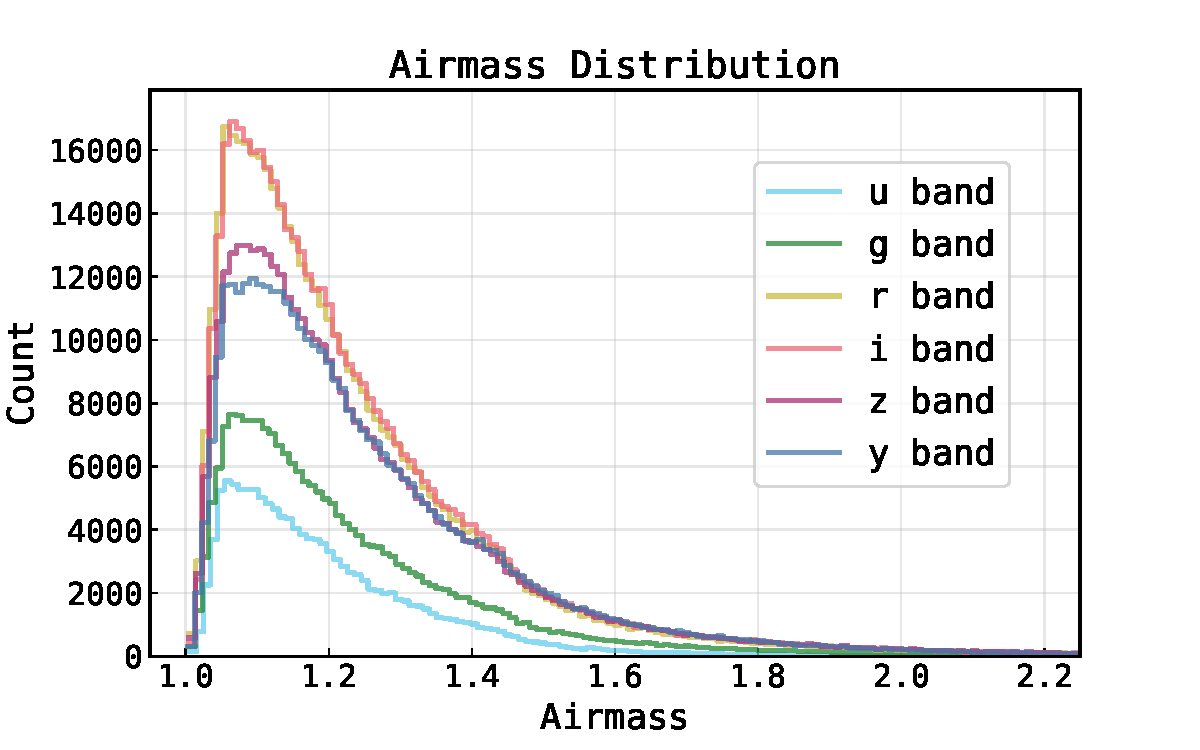
\includegraphics[width=0.43\textwidth]{figures/baseline_v2_0_10yrs_Count_airmass_u_g_r_i_z_y_ONED_ComboBinnedData.pdf}
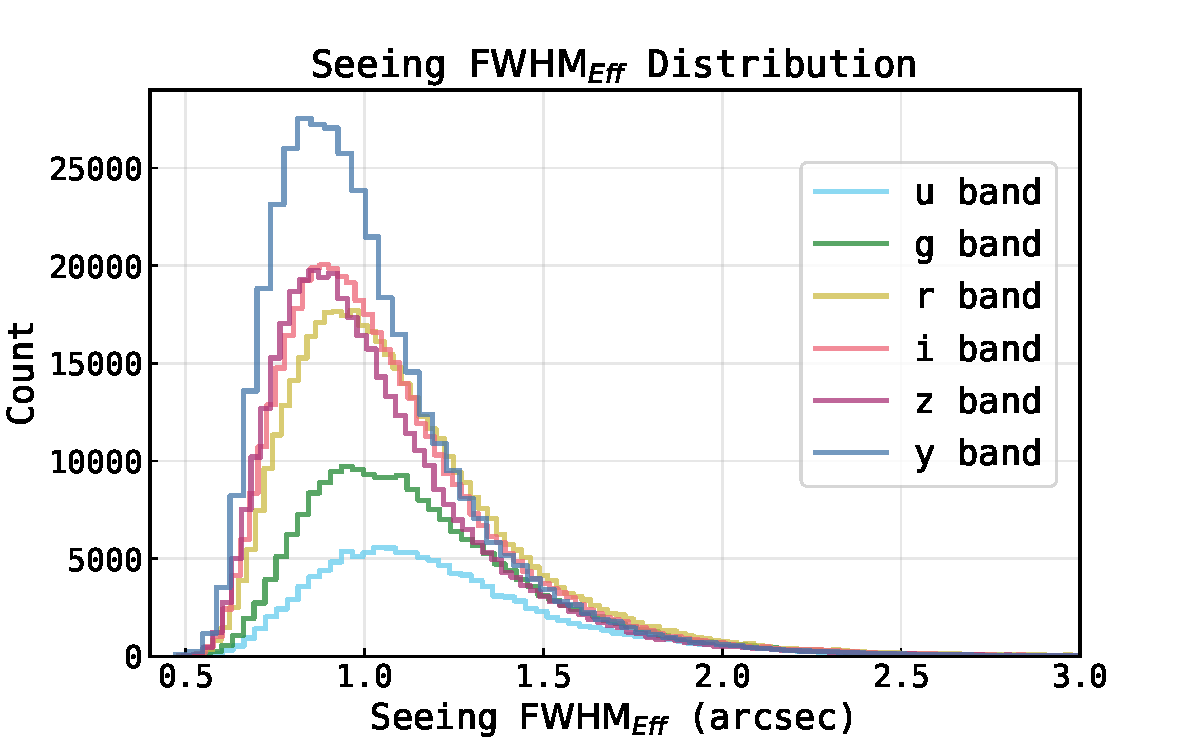
\includegraphics[width=0.43\textwidth]{figures/baseline_v2_0_10yrs_Count_seeingFwhmEff_u_g_r_i_z_y_ONED_ComboBinnedData.pdf}

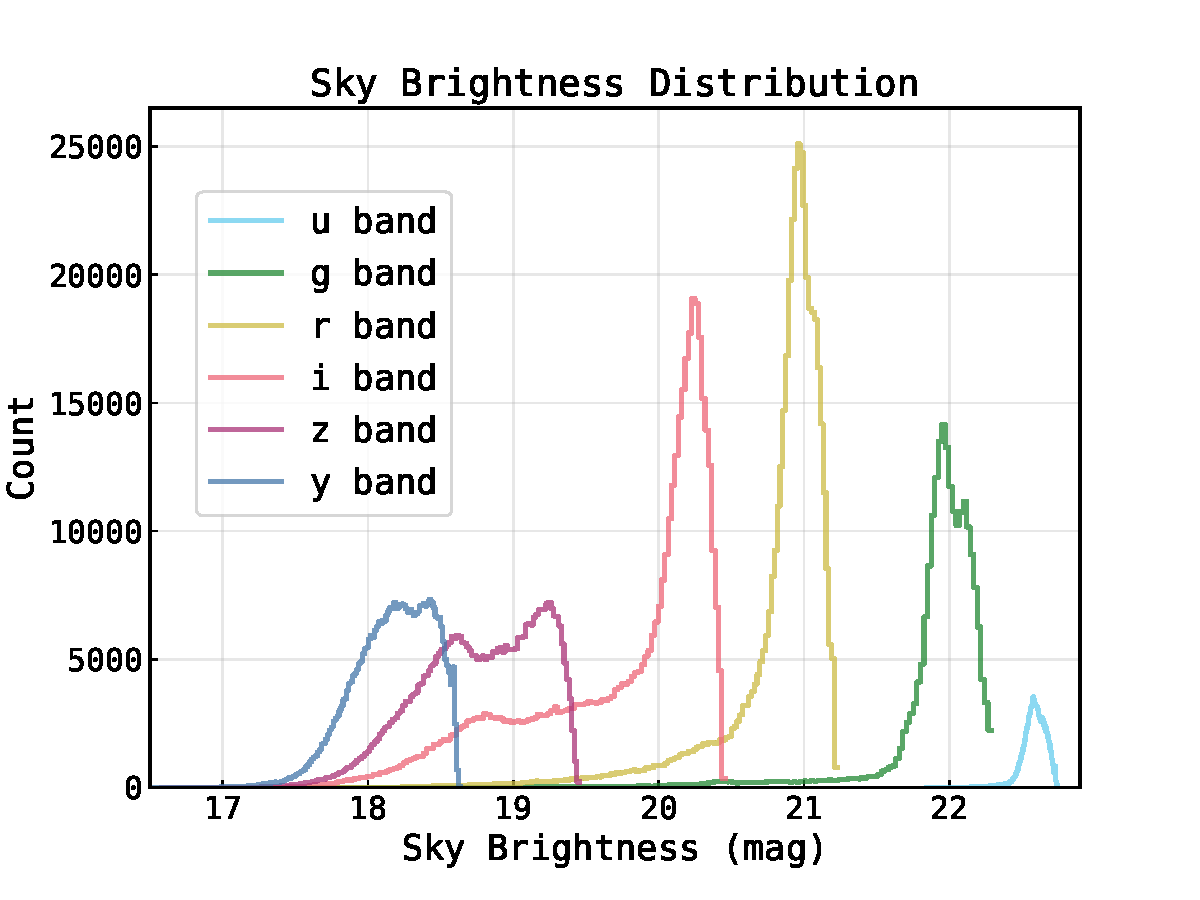
\includegraphics[width=0.43\textwidth]{figures/baseline_v2_0_10yrs_Count_skyBrightness_u_g_r_i_z_y_ONED_ComboBinnedData.pdf}
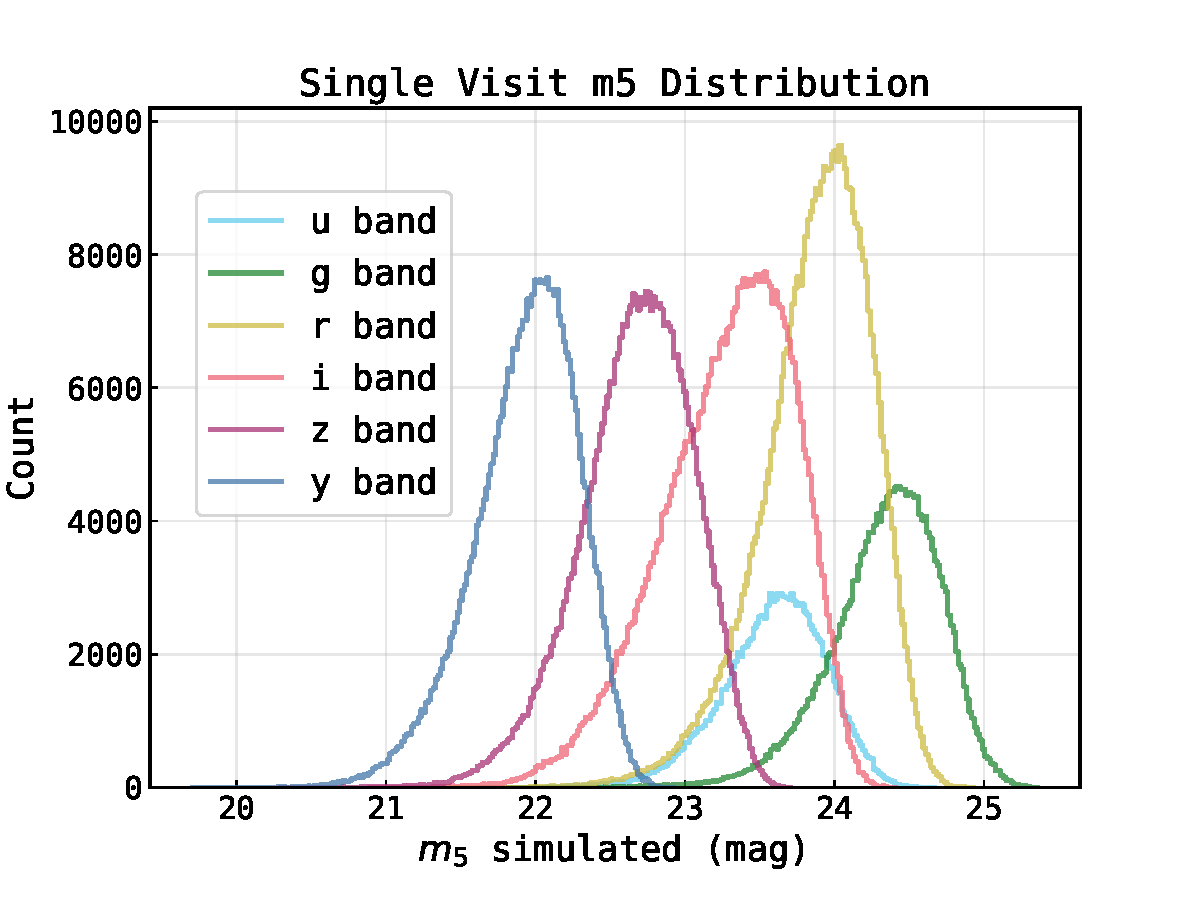
\includegraphics[width=0.43\textwidth]{figures/baseline_v2_0_10yrs_Count_fiveSigmaDepth_u_g_r_i_z_y_ONED_ComboBinnedData.pdf}
\caption{Distribution of airmass, seeing (\fwhme, see \autoref{sec:estdepth}), sky brightness, and \mf\ for the 10-year LSST survey simulated in \baseline, including Wide-Fast-Deep and minisurveys within.}\label{fig:bv2distributions}
\end{figure}
\FloatBarrier
\begin{table}
\caption{Simulated distributions of visit airmass, sky brightness, and seeing (\fwhme, see \autoref{sec:estdepth}) and their impact on \mf\ ($\Delta m$'s). The \mf\ reference is reported in row 1 in this table (same as \autoref{tab:bl1} row 8) for the reader's convenience. The \mf\ estimates resulting from survey simulations is reported for the \baseline\ LSST simulation. As these are calculated as medians over the 10-year simulation, small discrepancies between the reported \mf\ simulated median values and those obtained correcting the \mf\ reference values by the reported $\Delta m$ combined are expected.}\label{tab:bl2}
    \centering
\begin{tabular}{llrrrrrr}
\hline
{} &&      u &      g &      r &      i &      z &      y \\
\hline
\mf &reference %(X=1, median FWHM500, dark sky)
&  23.87 &  24.64 &  24.21 &  23.79 &  23.18 &  22.37 \\
\hline
\hline
airmass &reference                 &   1.00 &   1.00 &   1.00 &   1.00 &   1.00 &   1.00 \\
 &25th percentile       &   1.09 &   1.10 &   1.10 &   1.10 &   1.11 &   1.11 \\
 &median                &   1.16 &   1.18 &   1.18 &   1.18 &   1.19 &   1.20 \\
 &75th percentile       &   1.27 &   1.31 &   1.31 &   1.32 &   1.33 &   1.34 \\
\hline
sky brightness& reference           &  22.68 &  22.11 &  21.11 &  20.39 &  19.43 &  18.63 \\
 &25th percentile &  22.54 &  21.87 &  20.78 &  19.33 &  18.48 &  17.99 \\
& median          &  22.59 &  21.98 &  20.94 &  20.01 &  18.80 &  18.20 \\
 &75th percentile &  22.64 &  22.10 &  21.03 &  20.23 &  19.13 &  18.39 \\
\hline
seeing \fwhme& reference             &   1.04 &   0.98 &   0.92 &   0.88 &   0.86 &   0.84 \\
 &25th percentile &   0.97 &   0.93 &   0.88 &   0.85 &   0.83 &   0.82 \\
 &median          &   1.16 &   1.11 &   1.05 &   1.01 &   0.97 &   0.95 \\
 &75th percentile &   1.41 &   1.34 &   1.27 &   1.22 &   1.18 &   1.14 \\

\hline
%{} &      u &      g &      r &      i &      z &      y \\
\hline
 &25th percentile       &   -0.05 &   -0.02 &   -0.01 &   -0.01 &   -0.01 &   -0.02 \\
$\Delta m$ airmass &median                &   -0.08 &   -0.04 &   -0.02 &   -0.02 &   -0.01 &   -0.03 \\
&75th percentile       &   -0.13 &   -0.07 &   -0.04 &   -0.03 &   -0.02 &   -0.06 \\
\hline
 &25th percentile &   -0.07 &   -0.12 &   -0.17 &   -0.53 &   -0.48 &   -0.32 \\
$\Delta m$ sky brightness& median          &   -0.04 &   -0.07 &   -0.09 &   -0.19 &   -0.31 &   -0.22 \\
 &75th percentile &   -0.02 &   -0.01 &   -0.04 &   -0.08 &   -0.15 &   -0.12 \\
\hline
&25th percentile &  0.08 &  0.05 &  0.05 &  0.04 &  0.03 &  0.03 \\
$\Delta m$ seeing \fwhme &median          &   -0.12 &   -0.14 &   -0.14 &   -0.14 &   -0.14 &   -0.14 \\
 &75th percentile &   -0.33 &   -0.35 &   -0.34 &   -0.35 &   -0.35 &   -0.34 \\
 \hline
 $\Delta m$ {combined} &median          &   -0.24 &   -0.25 &   -0.25 &   -0.35 &   -0.46 &   -0.39 \\

\hline
\hline
\mf\ & simulated, median                      &  23.62 &  24.38 &  23.92 &  23.34 &  22.70 &  21.97 \\
\hline

\hline
\end{tabular}
\end{table}


 \FloatBarrier


\subsection{Realistic per-amplifier characteristics and related corrections}\label{sec:per-amp}
In all of the work described above, the read-noise and Quantum Efficiency (QE) curve have been assumed to be constant across the entire focal plane. In reality, each CCD chip will have slightly different QE curves and each amplifier will have a different read-noise value. Notably, Rubin's camera uses CCD chips produced by two different vendors, which have different characteristic QE and read-noise values.  As mentioned earlier, assuming 8.8 e$^-$/pixel/read-out as the single read-noise value is a conservative choice as the median noise per amp is significantly lower (\autoref{fig:rndist}). The QE values used in the presented calculations assume a ``joint'' vendor QE curve, which is defined as the minimum QE value at each wavelength; as such, it does not truly represent the expected performance as a function of wavelength for either vendor, but rather the likely most conservative estimate. Vignetting effects also impact the limiting magnitudes near the edges of the field of view, and this effect has not been taken into account in the calculations presented thus far. For the filter throughput curves, the filter requirements, encoded in the \href{https://github.com/lsst-pst/syseng_throughputs}{{\tt syseng\_throughputs}}, are adopted.

As CCDs have been delivered to the project, measurements of the expected read-noise, QE curves, and vignetting have been carried out for each amplifier. While incorporating these per-amp measurements in the 10-year survey simulations would be computationally impractical, slowing down the simulations significantly, their effect can be encoded through \autoref{eq:Cm} and \autoref{eq:dCm} applied to the \mf\ reference from which the simulations are derived, assuming median values. Applying $\Delta m$ combined (as shown in \autoref{tab:bl2}) as an additive factor to the ``\mf\ reference, corrected'' values reported in \autoref{tab:bl3} would lead to a new,  ``\mf\ simulated corrected'', representing the final expected single-image depths based on \baseline\ (reported in \autoref{tab:bl3}).

The distribution of read-noise for all camera amplifiers is shown in \autoref{fig:rndist} and the correction associated with read-noise, QE, as well as vignetting effects is shown in terms of $\Delta C_m$ in \autoref{fig:ccdplane} for each amplifier in the CCD plane in the $u$ and $y$ bands (where the effects are most and least significant, respectively).
The per filter corrections applied to \mf\ reference via \autoref{eq:Cm} and \autoref{eq:dCm} (including the QE and vignetting in $\Delta C_m^\infty$), are also reported in \autoref{tab:bl3}, as well as how they propagate to \mf\ simulated.

\FloatBarrier

\begin{table}\caption{Corrections associated with per-amp read-noise, QE, and vignetting, their mean values and Inter-Quartile Range (IQR) across the CCD plame, and their impact on \mf\ reference and \mf\ simulated.}\label{tab:bl3}
    \centering
 \begin{tabular}{llrrrrrr}
 \hline
 {} & &             u &      g &  r &   i &     z &      y \\
\hline
\mf &  reference &  23.87 &  24.64 &  24.21 &  23.79 &  23.18 &  22.37 \\
\hline
\hline
\cm & reference &  23.46 &  24.45 &  24.45 &  24.35 &  24.19 &  23.75 \\
 &per amp median       &  23.64 &  24.58 &  24.56 &  24.42 &  24.23 &  23.75 \\
& per amp IQR          &   0.15 &   0.08 &   0.08 &   0.04 &   0.03 &   0.06 \\
\hline
 $\Delta C_m^\infty$ & reference       &   0.28 &   0.15 &   0.09 &   0.06 &   0.04 &   0.03 \\
 & per amp median  &   0.15 &   0.07 &   0.04 &   0.03 &   0.02 &   0.02 \\
 & per amp IQR     &   0.07 &   0.03 &   0.02 &   0.01 &   0.01 &   0.00 \\
  \hline
  \hline
\mf & reference, corrected       &  24.05 &  24.77 &  24.32 &  23.86 &  23.22 &  22.37 \\
&simulated median, corrected    &  23.80 &  24.50 &  24.03 &  23.41 &  22.74 &  21.96 \\
\end{tabular}
\end{table}
\FloatBarrier
\clearpage

\FloatBarrier
\begin{figure}[!ht]
\centering
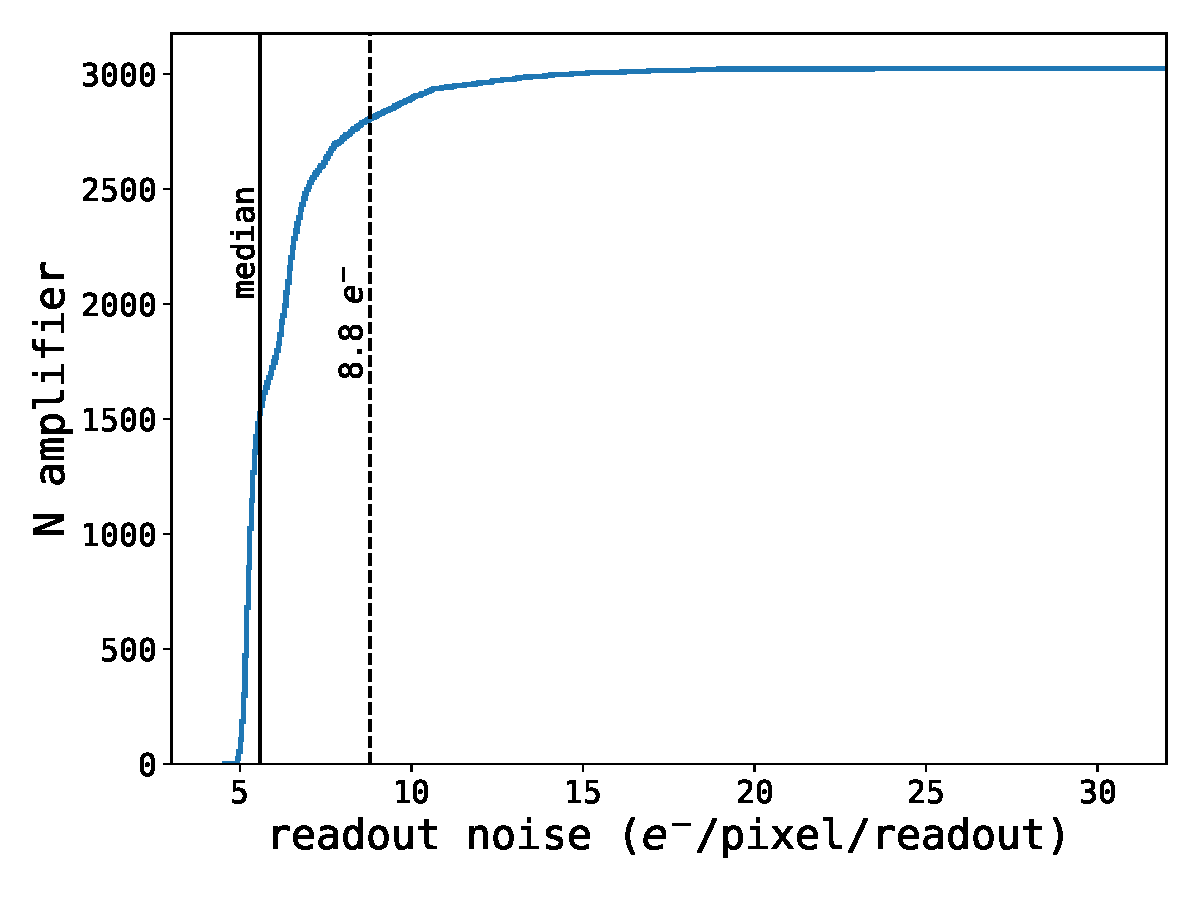
\includegraphics[width=0.53\textwidth]{figures/ampnoise.pdf}
\caption{Readout noise cumulative distribution for the 3024 CCD segments (aka amplifiers) on the focal plane of the Camera. The values are from Camera test run 13283, using bias images taken using Version 26 of the sequencer, with the full camera in operation and analyzed with the Camera \href{https://github.com/lsst-camera-dh/eotest}{EOTest package}. This run was also used for Camera Requirement Verification. The median noise is measured to be $\sim$5.5~$e^-$/pixel/readout, well below the requirement of 9~$e^-$/pixel/readout. The distribution shows a tail with 95\% of the amplifiers within 9~$e^-$/pixel/readout. Vertical lines mark the median and nominal 9~$e^-$/pixel/readout noise values. One bad segment is not shown in the distribution.}\label{fig:rndist}
\end{figure}


\FloatBarrier
 \FloatBarrier


\begin{figure}[!hb]
    \centering

    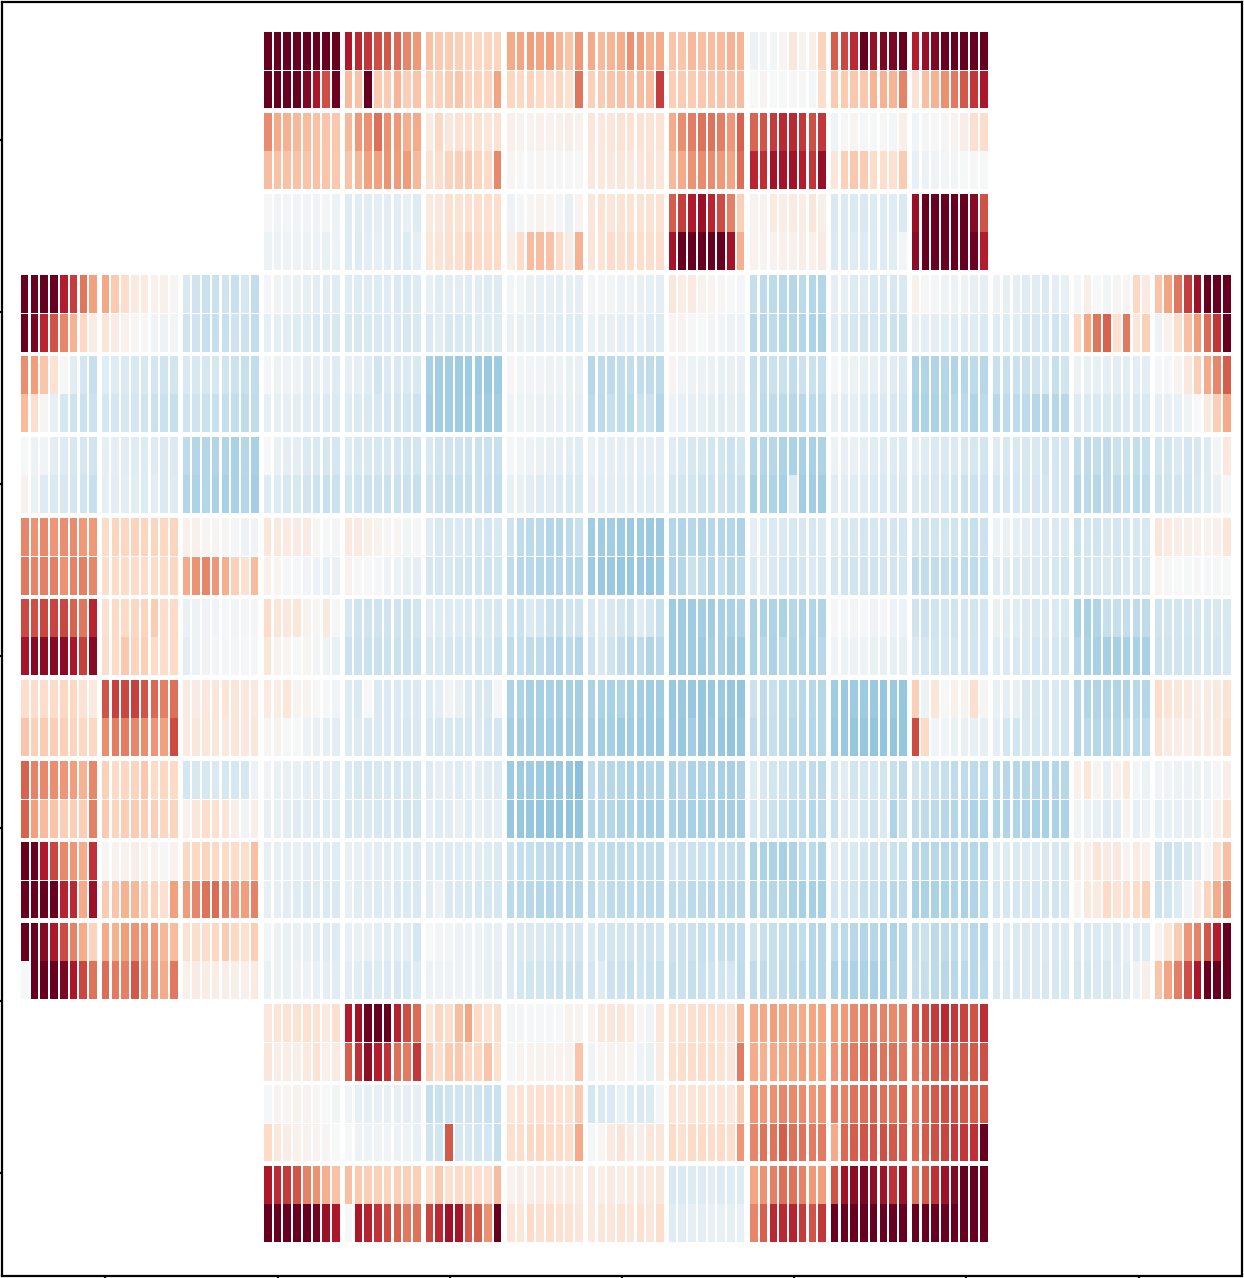
\includegraphics[width=0.35\textwidth]{figures/ccdplaneU}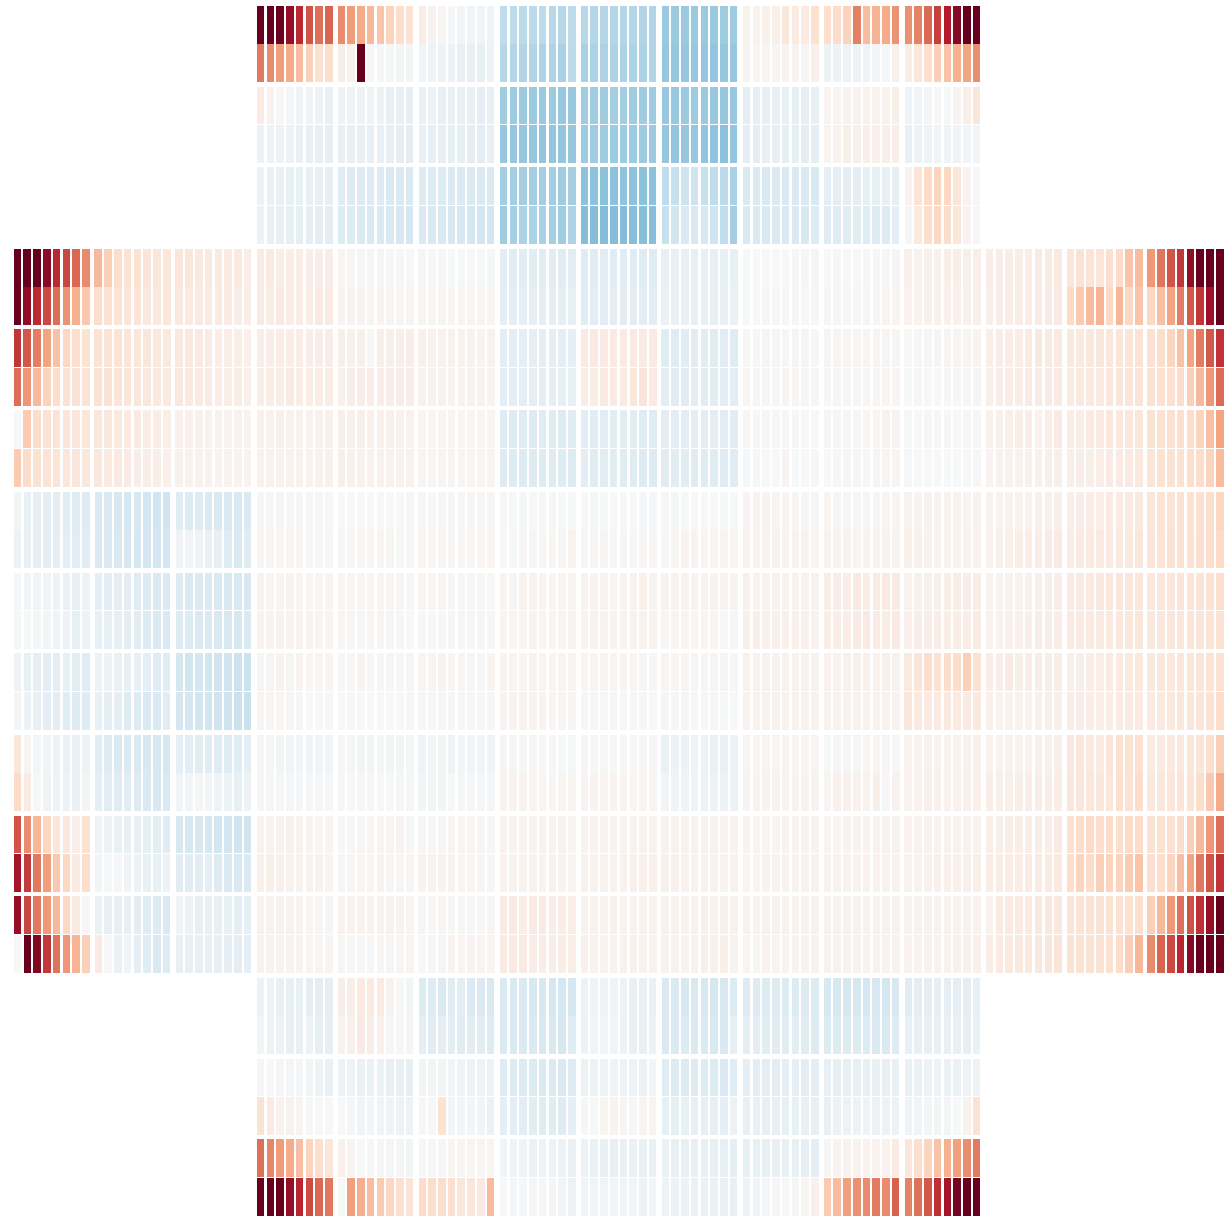
\includegraphics[width=0.35\textwidth]{figures/ccdplaneY}
\includegraphics[height=0.36\textwidth]{figures/colorbar.png}
\caption{The $u$ (left) and $y$ band (right) $\Delta Cm$ corrections associated with read-noise, QE, and vignetting effects for each amplifier in the LSST DOE Camera CCD plane. The $u$ and $y$ bands represent the most extreme and most modest correction and correction IQR values, respectively (see \autoref{tab:bl3}).}\label{fig:ccdplane}
\end{figure}
 \FloatBarrier


%\FloatBarrier



\subsection{Co-added depth distribution}\label{sec:coadd}

With the survey simulations in hand, we can calculate the expected coadded depth in each band. The final coadded depth is dependent on the number of visits acquired at any point in the sky, as well as on the individual image depths. These quantities are strongly dependent on survey strategy, although they are flexible within the limitations set by the total survey lifetime, minimum survey area, and observing duty-cycle requirements. Table 24 of the SRD reports an illustrative example of the LSST number of visits per bandpass and the corresponding idealised coadded depth of the survey, consistent with the assumption of a single image \mf\ values as reported in Table 6 of SRD (and included in \autoref{tab:SRDm5}, row 1, of this document).  We can now update these values with current survey simulations and using a realistic disstribution of \mf\ values calculated as described above.

There is a trade-off between the total number of visits per field and the area covered to a specified depth.
The SRD\ specifies minimum and design values for both the area covered and the median number of visits per pointing over that area in Tables 22 and 23: minimum values corresponding to a median of 750 visits per pointing over 15,000 sq. degrees, and design values of 825 visits per pointing over 18,000 sq. degrees. This footprint and the corresponding survey are referred to as the ``Wide Fast Deep'', hereafter WFD. In  \baseline, 18,620 sq. degrees of sky receive at least 750 observations, with a median value of 829 visits per pointing over the same area.  Conversely, an 18,000 square degree area receives a median of 839 visits.
This represents an increase in footprint and number of visits over the illustrative values stated in the SRD. The per-band median number of visits per pointing over the 18,620 sq. degree WFD footprint are listed in \autoref{tab:wfd_nvis}, together with the resulting coadded depths calculated using the pointing histories simulated in \baseline.


  As part of the SCOC work to define the survey footprint used for \baseline, trades between total area covered and number of visits per pointing were considered (see \citeds{PSTN-053}). The current footprint represents the result of this optimization and meets and exceeds the design requirements.
  These depths are consistent with the median individual image depths from \autoref{tab:bl1}, scaled by the median number of visits per pointing, reinforcing that most visits are obtained in or near median conditions.

\FloatBarrier

\begin{table}[h!]
\caption{WFD visits per pointing and coadded  depths. The 10-year LSST depth is reported as the median across all fields in the survey footprint in \baseline\ before and after correcting for the read-noise, QE, and vignetting effects as they vary across the CCD plane (see \autoref{tab:bl3} and  \autoref{sec:per-amp})}\label{tab:wfd_nvis}
\small
    \centering
\begin{tabular}{llrrrrrr}
\hline
{} & &    u &     g &      r &      i &      z &      y \\
\hline
number of visits &25th percentile &  53.0 &  70.0 &  178.0 &  181.0 &  160.0 &  164.0 \\
&   median       &  56.0 &  74.0 &  184.0 &  187.0 &  166.0 &  171.0 \\
& 75th percentile &  59.0 &  78.0 &  190.0 &  193.0 &  173.0 &  178.0 \\
\hline
\mf\ median coadded &         &  25.4 &  26.8 &   26.8 &   26.3 &   25.6 &   24.8 \\
\hline
\mf\ median coadded corrected&         &  25.6 &  26.9 &   26.9 &   26.4 &   25.6 &   24.8 \\
\end{tabular}
\end{table}

\FloatBarrier

%This corresponds to a median of 838 total visits. This value is between the {\it design} (845) and {\it minimum} (750) specifications included in the SRD, but with an increase in sky coverage.


\section{Further optimization options}\label{sec:optimize}

The \mf\ estimates reported in \autoref{tab:bl2} can be further optimized, if desired, to increase the per visit or coadded depth of the survey.



 As discussed in \autoref{sec:SRD}, exposure time could be reassigned between
bands. This would increase the \mf\ in some bands, at the cost of a decrease in others.

 A substantive fraction of the visits in \baseline\ were, in fact, collected as part of mini-surveys (see LSST Overview paper; \citet{2019ApJ...873..111I}), and these observations could be redirected, if desired, to cover the WFD footprint in the main LSST survey, thus increasing the coadded \mf. In the \baseline, the fraction of images collected as part of surveys other than the WFD corresponds to about  $\sim34\%$. This implies that, in principle, the \baseline\ WFD has a ``reserve'' corresponding to $\sim280$ images per field.  The decision of reassigning these images to the WFD requires analyzing and balancing  science priorities, and the SCOC is charged with performing this balancing exercise. Similarly, the distribution of visits between filters is under consideration by the SCOC.  The distribution shown in \autoref{tab:wfd_nvis} reflects current SCOC guidance, and also generally matches the illustrative distribution provided in Table 24 of the SRD.


The derived estimates of \mf\ presented in \autoref{tab:bl1} assume two exposures per visit to a combined $t_{vis}=30$~seconds, except in $u$ band. Abolishing the two-snap strategy would provide an improvement in efficiency via a decrease in overtime by about 8\%. This time could be used to increase the observed footprint, the number of visits for pointing, or the total exposure in all or some bands. Each one of these choices, however, should also be vetted against the resulting image quality, image processing requirements, and overall scientific throughput of the survey.

Finally, the reported expected \mf\ values assume current estimates of the mirrors' reflectivities, as discussed in \autoref{sec:SRD}, which are still being optimized, filter coating transmission functions which will soon be updated with as-built measurements, as well as a surveying efficiency that remains to be demonstrated after the observatory is completed and enters its operations phase.

% You can also use the \input command to include several content files.

\appendix
% Include all the relevant bib files.
% https://lsst-texmf.lsst.io/lsstdoc.html#bibliographies
\section{References} \label{sec:bib}
\renewcommand{\refname}{} % Suppress default Bibliography section
\bibliography{local,lsst,lsst-dm,refs_ads,refs,books}

% Make sure lsst-texmf/bin/generateAcronyms.py is in your path
\section{Acronyms} \label{sec:acronyms}
\addtocounter{table}{-1}
\begin{longtable}{p{0.145\textwidth}p{0.8\textwidth}}\hline
\textbf{Acronym} & \textbf{Description}  \\\hline

B & Byte (8 bit) \\\hline
CCD & Charge-Coupled Device \\\hline
DIMM & Differential Image Motion Monitor \\\hline
DOE & Department of Energy \\\hline
FWHM & Full Width at Half-Maximum \\\hline
HTML & HyperText Markup Language \\\hline
LPM & LSST Project Management (Document Handle) \\\hline
LSE & LSST Systems Engineering (Document Handle) \\\hline
LSST & Legacy Survey of Space and Time (formerly Large Synoptic Survey Telescope) \\\hline
M1 & primary mirror \\\hline
M2 & Secondary Mirror \\\hline
M3 & tertiary mirror \\\hline
PSF & Point Spread Function \\\hline
PST & Project Science Team \\\hline
PSTN & Project Science Technical Note \\\hline
QE & quantum efficiency \\\hline
RTN & Rubin Technical Note \\\hline
SCOC & Survey Cadence Optimization Committee \\\hline
SED & Spectral Energy Distribution \\\hline
SNR & Signal to Noise Ratio \\\hline
SRD & LSST Science Requirements; LPM-17 \\\hline
WFD & Wide Fast Deep \\\hline
arcsec & arcsecond second of arc (unit of angle) \\\hline
\end{longtable}

% If you want glossary uncomment below -- comment out the two lines above
%\printglossaries





\end{document}
